\documentclass[border=2pt]{standalone}
\usepackage{tikz}
\usetikzlibrary{datavisualization.formats.functions,datavisualization.polar}
\newcount\ticknumber
\newcommand{\probetick}{%
  \global\advance\ticknumber by1
  \pgfextractx{\dimen0}{\pgfpointanchor{\tikzlastnode}{center}}%
  \pgfextracty{\dimen2}{\pgfpointanchor{\tikzlastnode}{center}}%
  \typeout{POLAR-TICK \the\ticknumber: x=\the\dimen0, y=\the\dimen2}}
\tikzdatavisualizationset{every ticks/.append style={node style={append after command={\pgfextra{\probetick}}}}}
\begin{document}
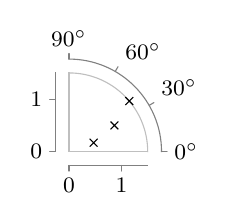
\begin{tikzpicture}
  \datavisualization [scientific polar axes={clean,0 to 90},
    angle axis={ticks={step=30}},radius axis={length=1cm,ticks={step=1}},visualize as scatter]
    data point [angle=20,radius=.5]
    data point [angle=30,radius=1]
    data point [angle=40,radius=1.5];
\end{tikzpicture}
\end{document}
